%%%%%%%%%%%%%%%%%%%%%%%%%%%%%%%%%%%%%%%%%%%%%%%%%%%%%%%%%%%%%%%%%
\chapter{INTRODUCTION}\label{introduction}
%%%%%%%%%%%%%%%%%%%%%%%%%%%%%%%%%%%%%%%%%%%%%%%%%%%%%%%%%%%%%%%%%
Lorem ipsum dolor sit amet, consectetur adipiscing elit. Praesent imperdiet, nisi 
nec aliquam cursus, dui turpis mollis nisl, ac consequat tellus sapien sit amet 
magna. Duis vel venenatis velit. Vestibulum ante ipsum primis in faucibus orci 
luctus et ultrices posuere cubilia Curae; Proin malesuada risus nec metus dapibus 
eu tincidunt lectus dignissim. 

\section{Purpose of Thesis}\label{purposeofthesis}

Lorem ipsum dolor sit amet, consectetur adipiscing elit. Praesent imperdiet, nisi 
nec aliquam cursus, dui turpis mollis nisl, ac consequat tellus sapien sit amet 
magna. Duis vel venenatis velit. Vestibulum ante ipsum primis in faucibus orci 
luctus et ultrices posuere cubilia Curae; Proin malesuada risus nec metus dapibus 
eu tincidunt lectus dignissim. 

\section{Literature Review}\label{literaturereview}
Object Recognition over mobile devices is done using different methods. The main approach is to extract features, create a feature vector out of them and a learning algorithm to recognize the pattern. This is done in two different architecture \cite{residual_enhanced_visual_vector}, first mobile device extract feature vector and send it to a server that Database is based on and detecting procedure done over server and the other approach is to do all processes over mobile device itself. \\
Feature extraction process mainly done with different algorithms like SIFT\cite{SIFT}, SURF\cite{SURF}, GLOH\cite{GLOH} and HOG\cite{HOG}. The other problem is to extract feature vector out of this features (indexing) that is done by Bag of Words\cite{BoW}, Vocabulary Trees \cite{vocabulary_tree} and more recently by Residual Enhanced Visual Vectors(REVV) \cite{residual_enhanced_visual_vector}. The other approach for extracting features and presenting them is using unsupervised learning methods that include deep learning methods. Deep Learners are Artificial Neural Networks (ANN) that have more than 2 hidden layers. In this hidden layers our network tries to represent data with simpler features mainly using unsupervised learning approach \cite{DBN}. The most successful and famous deep networks at visual detection are Deep Belief Network (DBN) \cite{DBN}, Convolutional Neural Networks (CNN) \cite{CNN} and Convolutional Deep Belief Network (CDBN) \cite{CDBN}. That are extremely successful at recent years and pretty dominate Content Based Image Retrieval.
\begin{figure}
 \centering
 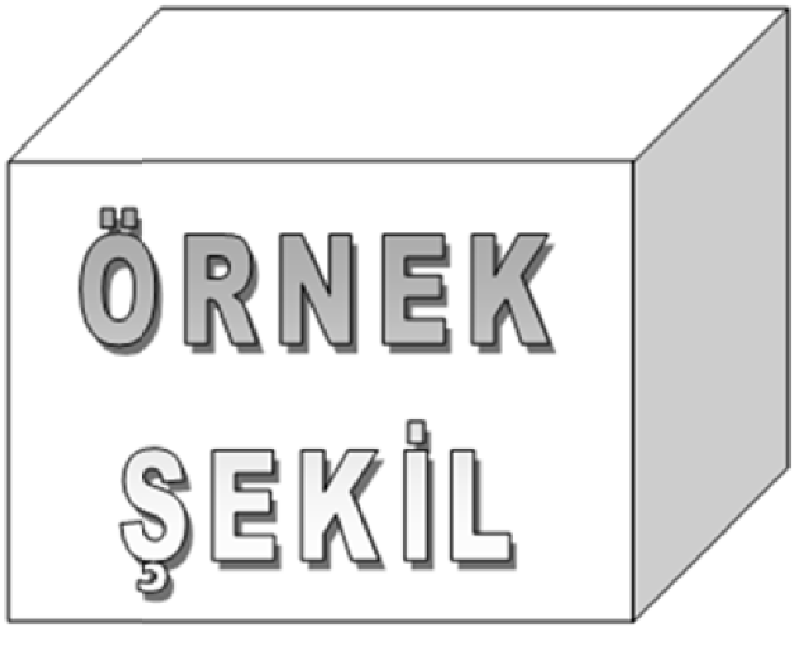
\includegraphics[width=10cm,keepaspectratio=true]{./fig/sekil1}
 % sekil1.eps: 0x0 pixel, 300dpi, 0.00x0.00 cm, bb=14 14 592 479
 \caption{Model structures.}
\end{figure}

\section{Hypothesis}

Lorem ipsum dolor sit amet, consectetur adipiscing elit. Praesent imperdiet, nisi 
nec aliquam cursus, dui turpis mollis nisl, ac consequat tellus sapien sit amet 
magna. Duis vel venenatis velit. Vestibulum ante ipsum primis in faucibus orci 
luctus et ultrices posuere cubilia Curae; Proin malesuada risus nec metus dapibus 
eu tincidunt lectus dignissim. 

Lorem ipsum dolor sit amet, consectetur adipiscing elit. Praesent imperdiet, nisi 
nec aliquam cursus, dui turpis mollis nisl, ac consequat tellus sapien sit amet 
magna. Duis vel venenatis velit. Vestibulum ante ipsum primis in faucibus orci 
luctus et ultrices posuere cubilia Curae; Proin malesuada risus nec metus dapibus 
eu tincidunt lectus dignissim. 

Lorem ipsum dolor sit amet, consectetur adipiscing elit \cite{Onur_Calikus_YLT}. Praesent imperdiet, nisi 
nec aliquam cursus, dui turpis mollis nisl, ac consequat tellus sapien sit amet 
magna. Duis vel venenatis velit. Vestibulum ante ipsum primis in faucibus orci 
luctus et ultrices posuere cubilia Curae; Proin malesuada risus nec metus dapibus 
eu tincidunt lectus dignissim \cite{unesco}.

Lorem ipsum dolor sit amet, consectetur adipiscing elit. Praesent imperdiet, nisi 
nec aliquam cursus, dui turpis mollis nisl, ac consequat tellus sapien sit amet 
magna. Duis vel venenatis velit. Vestibulum ante ipsum primis in faucibus orci 
luctus et ultrices posuere cubilia Curae; Proin malesuada risus nec metus dapibus 
eu tincidunt lectus dignissim.Lorem ipsum dolor sit amet, consectetur adipiscing elit. 
Praesent imperdiet, nisi nec aliquam cursus, dui turpis mollis nisl, ac consequat 
tellus \cite{mccaffrey88} \cite{moore91} \cite{nelson88}
\cite{sisaky} \cite{simpsondvd} \cite{startrek} \cite{TS-40561} \cite{url-1} \cite{url-2}
\cite{vanden2001}.

Duis vel venenatis velit. Vestibulum ante ipsum primis in faucibus orci 
luctus et ultrices posuere cubilia Curae; Proin malesuada risus nec metus dapibus 
eu tincidunt lectus dignissim.

Lorem ipsum dolor sit amet, consectetur adipiscing elit. Praesent imperdiet, nisi 
nec aliquam cursus, dui turpis mollis nisl, ac consequat tellus sapien sit amet 
magna. Duis vel venenatis velit. Vestibulum ante ipsum primis in faucibus orci 
luctus et ultrices posuere cubilia Curae; Proin malesuada risus nec metus dapibus 
eu tincidunt lectus dignissim.

\begin{table*}
{\setlength{\tabcolsep}{14pt}
\caption{Table captions must be ended with a full stop.}
\begin{center}
\vspace{-6mm}
\begin{tabular}{cccc}
\hline\hline
Column A & Column B & Column C & Column D \\
\hline
Row A & Row A & Row A & Row A \\
Row B & Row B & Row B & Row B \\
Row C & Row C & Row C & Row C \\
\hline
\end{tabular}
\vspace{-6mm}
\end{center}
\label{sitable3}}
\end{table*}

Lorem ipsum dolor sit amet, consectetur adipiscing elit. Praesent imperdiet, nisi 
nec aliquam cursus, dui turpis mollis nisl, ac consequat tellus sapien sit amet 
magna. Duis vel venenatis velit. Vestibulum ante ipsum primis in faucibus orci 
luctus et ultrices posuere cubilia Curae; Proin malesuada risus nec metus dapibus 
eu tincidunt lectus dignissim \cite{1993JHyd..144..193B}.


